%% DONE
\id{МРНТИ 52.31.29}{}

\begin{articleheader}
\sectionwithauthors{A.T. Тұрғали, Қ.Ә. Қожахмет, А.Г. Гусманова}{ГЕОЛОГИЧЕСКАЯ И ПОИСКОВАЯ ИЗУЧЕННОСТЬ УЧАСТКА ОРДАБАСЫ С ЦЕЛЬЮ ПОИСКОВО-ОЦЕНОЧНЫХ РАБОТ НА МЕДНУЮ РУДУ И ПОПУТНЫЕ КОМПОНЕНТЫ}

{\bfseries
A.T. Тұрғали\textsuperscript{\envelope } \authorid,
Қ.Ә. Қожахмет\authorid,
А.Г. Гусманова\authorid}
\end{articleheader}

\begin{affiliation}
\emph{Каспийский университет технологии и инжиниринга им. Ш. Есенова, Актау, Казахстан}

\raggedright \textsuperscript{\envelope }{\em Корреспондент- автор: \href{mailto:aiman.tt@mail.ru}{\nolinkurl{aiman.tt@mail.ru}}}
\end{affiliation}

В данной статье исследуется геологическая и поисковая характеристика
участка Ордабасы с акцентом на поисково-оценочные работы по медной руде
и сопутствующим компонентам. Площадь исследования составляет 15 км², и,
хотя участок проявляет перспективность, окончательная оценка не была
проведена из-за недостатка поисково-оценочных работ для формирования
промышленных запасов меди и сопутствующих компонентов, при этом
прогнозные ресурсы классифицируются по категории Р3. Первоначальные
геологические исследования данной территории проводились в 1938-1946
годах и были связаны с изучением Атасуйских железорудных месторождений.
В ходе этих работ были составлены геологические карты северной части
Атасуйского рудного поля, а также геоморфологические карты и карты
окрестностей Малого Ктая. Впервые в регионе выделены горизонты нижнего
девона: каражирикский, прибалхашский и сарджальский. Также была
фаунистически охарактеризована тектурмасская свита кембрия, а
допалеозойские отложения разделены на свиты и пачки. Определены
перспективы на золото, медь и полиметаллы, а в фаменских отложениях
установлены фации, потенциально перспективные для поиска
свинцово-цинковых руд стратиформного типа. На основе обширных
картографических и поисковых работ были построены карты допалеозойских
образований, дробно расчленены отложения франского, фаменского ярусов и
нижнетурнейских отложений с выделением мелководных и глубоководных
фаций. Проведено геохимическое исследование района, выявлены новые
проявления рудной минерализации, что обосновало необходимость оценки
глубоких горизонтов медного месторождения Успенское. Поисковые работы
осуществлялись как в процессе геолого-съемочных работ, так и в ходе
специализированных поисков, что привело к выявлению редкометалльной и
медной минерализации, связанной с малой линейной интрузией гранитов.
Выделена значительная площадь минерализованных пород, что стало
основанием для продолжения поисковых работ на участке Просторненский.
Оценка оруденения проводилась с использованием различных методов,
включая магниторазведку и электроразведку. На площади также обнаружены
геофизические аномалии, связанные с эндо-экзоконтактом гранитоидов
Просторненского массива и осадочных пород нижнего силура. Большинство
этих аномалий изучено недостаточно или не проверено вовсе.

{\bfseries Ключевые слова:} геологическая изученность, руда, тектоника,
геологическое развитие, геофизика, аномалия, медь.

\begin{articleheader}
{\bfseries МЫС КЕНІ МЕН ІЛЕСПЕ КОМПОНЕНТТЕРГЕ ІЗДЕУ-БАҒАЛАУ ЖҰМЫСТАРЫ МАҚСАТЫНДА ОРДАБАСЫ УЧАСКЕСІНІҢ ГЕОЛОГИЯЛЫҚ ЖӘНЕ ІЗДЕСТІРУ ЗЕРДЕЛЕНУІ}

{\bfseries
А.Т.Тұрғали\textsuperscript{\envelope },
Қ.Ә. Қожахмет,
А.Г. Гусманова}
\end{articleheader}

\begin{affiliation}
\emph{Ш. Есенов атындағы Каспий технологиялар және инжиниринг университеті, Ақтау, Қазақстан,}

\emph{e-mail: aiman.tt@mail.ru}
\end{affiliation}

Бұл мақалада Ордабасы учаскесінің геологиялық және іздестіру сипаттамасы
зерттеліп, мыс кені мен ілеспе компоненттер бойынша іздестіру-бағалау
жұмыстарына екпін қойылады. Зерттеу алаңы 15 шаршы километр құрайды және
телім көріністі болғанымен, мыс пен онымен байланысты компоненттердің
өндірістік қорларын қалыптастыру үшін іздеу-бағалау жұмыстарының
болмауына байланысты түпкілікті бағалау жүргізілмеген, болжамды
ресурстар Р3 санатына жатқызылған. Бұл аумақтың алғашқы геологиялық
зерттеулері 1938-1946 жылдары жүргізілді және Атасу темір кен орындарын
зерттеумен байланысты болды. Осы жұмыстар барысында Атасу кен алқабының
солтүстік бөлігінің геологиялық карталары, сондай-ақ, Кіші Ктай
маңындағы геоморфологиялық карталары жасалды. Өңірде алғаш рет төменгі
девонның көкжиектері бөлінді: қаражирик, Балқаш және сарджал. Кембрий
Тектурмас формациясы да фауналық сипатта болды, ал палеозойға дейінгі
шөгінділер формациялар мен пакеттерге бөлінді. Алтын, мыс және
полиметалдар үшін болашақ көрініс анықталды, ал фамен шөгінділерінде
стратиформды типтегі қорғасын-мырыш кендерін іздеуге перспективалы
фациялар орнатылды. Кең ауқымды картографиялық және іздеу жұмыстарының
негізінде палеозойға дейінгі түзілімдердің карталары салынды, таяз және
терең теңіз фацияларын бөліп көрсете отырып, франк, фамен және төменгі
турнай шөгінділерінің шөгінділері бөлшектелді. Ауданға геохимиялық
зерттеу жүргізілді, кен минералдануының жаңа көріністері анықталды, бұл
Успенское мыс кен орнының терең көкжиектерін бағалау қажеттілігін
негіздеді. Іздеу жұмыстары геологиялық-түсірілім жұмыстары барысында да,
граниттердің шағын сызықтық интрузиясымен байланысты сирек металды және
мыс минералдануын анықтауға алып келген мамандандырылған іздеулер
барысында да жүзеге асырылды. Минералданған жыныстардың едәуір ауданы
бөлінді, бұл Просторненский учаскесінде іздеу жұмыстарын жалғастыруға
негіз болды. Кенденуді бағалау әртүрлі әдістерді, соның ішінде магниттік
барлау мен электр барлауды қолдану арқылы жүргізілді. Алаңда сонымен
қатар Просторненский массивінің гранитоидтары мен төменгі силурдың
шөгінді жыныстарының эндо-экзоконтактісіне байланысты геофизикалық
ауытқулар табылды. Бұл ауытқулардың көпшілігі жеткілікті зерттелмеген
немесе мүлдем тексерілмеген.

{\bfseries Түйін сөздер:} геологиялық зерттеу, кен, тектоника, геологиялық
даму, геофизика, аномалия, мыс.

\begin{articleheader}
{\bfseries GEOLOGICAL AND PROSPECTING STUDIES OF THE ORDABASY SITE FOR THE PURPOSE OF PROSPECTING AND EVALUATION WORKS FOR COPPER ORE AND ASSOCIATED COMPONENTS}

{\bfseries
A.T. Turgali\textsuperscript{\envelope },
K.A. Kozhakhmet,
A.G. Gusmanova}
\end{articleheader}

\begin{affiliation}
\emph{Caspian University of Technology and Engineering named after Sh. Yesenov, Aktau, Kazakhstan,}

\emph{e-mail: \href{mailto:aiman.tt@mail.ru}{\nolinkurl{aiman.tt@mail.ru}}}
\end{affiliation}

This article examines the geological and prospecting characteristics of
the Ordabasy site with an emphasis on prospecting and evaluation work on
copper ore and related components. The study area is 15 km2, and
although the site shows promise, a final assessment has not been carried
out due to a lack of prospecting and evaluation work to form industrial
reserves of copper and related components, while the forecast resources
are classified according to category P3. The initial geological studies
of this area were carried out in 1938-1946 and were associated with the
study of the Atasui iron ore deposits. In the course of these works,
geological maps of the northern part of the Atasui ore field, as well as
geomorphological maps and maps of the surroundings of the Small Altai
were compiled. For the first time in the region, the horizons of the
Lower Devonian are highlighted: Karazhirik, Balkhash and Sarjali. The
Texturmas formation of the Cambrian was also faunistically
characterized, and the Pre-Paleozoic deposits were divided into
formations and bundles. Prospects for gold, copper and polymetals have
been determined, and facies have been identified in the Famennian
deposits that are potentially promising for the search for lead-zinc
ores of the stratiform type. On the basis of extensive cartographic and
prospecting work, maps of pre-Paleozoic formations were constructed, the
deposits of the Fransk, Famensk tiers and Lower Turneian sediments were
fractionally dissected with the allocation of shallow and deep-water
facies. A geochemical study of the area was carried out, new
manifestations of ore mineralization were revealed, which justified the
need to assess the deep horizons of the Uspenskoye copper deposit.
Prospecting was carried out both in the process of geological survey
work and in the course of specialized searches, which led to the
identification of rare metal and copper mineralization associated with a
small linear intrusion of granites. A significant area of mineralized
rocks has been identified, which became the basis for the continuation
of prospecting work at the site of the Spacious. Mineralization was
assessed using various methods, including magnetic exploration and
electrical exploration. Geophysical anomalies associated with the
endo-exocontact of the granitoids of the Spacious massif and sedimentary
rocks of the Lower Silurian were also found on the area. Most of these
anomalies have not been sufficiently studied or verified at all.

{\bfseries Keywords:} geological study, ore, tectonics, geological
development, geophysics, anomaly, copper.

\begin{multicols}{2}
{\bfseries Введение.} Медная руда является важным сырьем для многих
отраслей, включая электронику, строительство и энергетическую
инфраструктуру. С увеличением потребления меди и других связанных
компонентов растёт необходимость в их разведке и добыче. При этом
исследование попутных компонентов, таких как золото или серебро, может
повысить экономическую эффективность проектов по добыче медной руды.
Таким образом, геологическая и поисковая изученность участка Ордабасы в
Карагандинской области Республики Казахстан является актуальной, а также
сочетает в себе научную новизну и практическую значимость в свете
глобальных тенденций в области ресурсов и экологии.

Исходя из этого, цель настоящей статьи заключается в исследовании
геологической и поисковой характеристики участка Ордабасы, с акцентом на
поисково-оценочные работы по медной руде и сопутствующим компонентам.
минералогических ресурсов, включая медь, золото, полиметаллы и редкие
металлы.

Для достижения поставленной цели сформулированы следующие задачи.

1. Оценка геологической изученности и характеристика геологического
строения района Ордабасы.

2. Анализ результатов поисково-оценочных работ, направленных на выявление
медных руд и сопутствующих компонентов.

3. Обзор исторических исследований и картографических материалов,
связанных с изучением участка.

4. Оценка перспективности продолжения поисковых работ на участке Ордабасы
на основе полученных данных.

В контексте выполнения этих задач, научная новизна данной работы
заключается в том, что в статье впервые проводится комплексная оценка
геологической структуры и минерализации участка Ордабасы с акцентом на
медь и редкие металлы, а также впервые систематизированы данные о
потенциальных перспективах региона для разработки меди, золота и
полиметаллических месторождений.

Пространственно-поисковая площадь расположена в Шетском районе
Карагандинской области. Площадь работ составляет 15
км\textsuperscript{2} Рассматриваемая площадь перспективна, но не
получила окончательной оценки из-за недостаточного количества
поисково-оценочных работ для формирования промышленных запасов меди и
попутных компонентов. Имеются прогнозные ресурсы по категории
Р\textsubscript{3}.

В своих работах В.Ф. Долгань в 1973 году {[}1{]} описал участок
следующим образом, участок Ордабасы расположен на площади листа
М-43-98-В. В 1973 году при ГС-50 листов М-43-98-А, Б, В, Г в пределах
интрузивного массива Итольген выявлено 4 пункта меднорудной
минерализации, отстоящих друг от друга на расстоянии 700-1500 метров.
Оруденение локализовано в массиве позднедевонских гранодиоритов, рудная
минерализация представлена зонами окварцевания и кварцевыми жилами с
малахитом, борнитом, халькопиритом и молибденитом. По зонам
минерализации были пройдены две канавы общей длиной 20 м и через весь
интрузивный массив пройдено два профиля магнито-электроразведочных
работ, в эндо- и экзоконтактах интрузии выявлены совмещенные
магнито-электроразведочные аномалии. Аномалии ВП имеют интенсивность 3\%
на фоне 1\%. В бороздовых пробах из канав содержание меди составляет
0,8-1,0\%, молибдена - до 0,2-0,4 \%, висмута - до 0,02 \%, серебра -
0,02 \%, золота - до 0,5 г/т.

Так, Ф.В. Долганем сделаны выводы:

1. рудная минерализация приурочена к неглубоко эродированной части
интрузивного массива;

2. зоны окварцевания в повышенных концентрациях содержат медь, молибден,
висмут;

3. в приконтактовых частях интрузивного массива выявлены магнитные и
электроразведочные аномалии, природа которых не изучалась;

4. в целом массив оценивается как перспективный на обнаружение
месторождений меди, редких и благородных металлов; рекомендуется
постановка поисковых геолого-геофизических работ.

{\bfseries Материалы и методы.} \emph{Геологическая изученность}{\bfseries .}
Центральный Казахстан представляет собой регион с разнообразными
залежами твердых полезных ископаемых. Здесь можно встретить залежи меди,
марганца, полиметаллов, золота, угля и железной руды. Природные ресурсы
способствую экономическому развитию не только региона, но и всего
Казахстана в целом. Из-за этого данный регион является объектом
пристального внимания ученых и геологов. Ученые активно изучают
геодинамическую позицию и минералогические особенности месторождений
данного региона Казахстана, что позволяет глубже понять процессы,
происходившие в недрах Земли. Исследования показывают, что образование
рудных тел связано с коллизией базальтовых островных дуг с
континентальными плитами, что могло привести к утолщению литосферы и
образованию богатых рудных тел. Так в статье Степанцева В.Г., Маката
Д.К. и Савельева Н.А. (2015) представлена геодинамиечская позиция
медно-порфирового меторождения Нурказган (Центральный Казахстан)
{[}2{]}. В научных трудах Бекжанова Г.Р. (2012) даны предварительные
предложения по соблюдению системности и стадийности при выборе
направлений геологоразведочных работ на медь {[}3{]}.

Сафонова И.Ю., Антонюк Р.М., Гурова А.В., Калугин В.М., Савинский И.А.,
Внуковский А.П., Орынбек Т.Ж. в статье «Геологическое строение и медное
оруденение Тектурмасского офиолитового пояса и смежных территорий
Центрального Казахстана» (2022) представили анализ ключевых этапов
магматической активности, связанных с формированием месторождений и
проявлений меди и других металлов {[}4{]}. Перспективы обнаружения
золото-медно-полиметаллического месторождения в Шешенкаринском рудном
поле в Центральном Казахстане показаны в работах Султанова Г.Д.,
Вихлянцева А.А. Исмаилова Х.К. (2019) {[}5{]}.

Исследованиями в области оценки восполнения запасов основных полезных
ископаемых занимались Гинатулин А.М., Дербас А.Н., Асанбаева У.Т.
(2016). Авторами было установлено что адекватное восполнение запасов
наблюдается лишь по железным рудам. В то же время, по нефти, газу,
хрому, меди, цинку, свинцу, титану, алюминию, золоту, серебру, бариту и
асбесту за последние десять лет не было достигнуто необходимого уровня
восполнения. Добыча этих ресурсов значительно превышает приросты запасов
и предполагает реализовывать ряд мероприятий, направленных на более
активное привлечение капитала в разведку и добычу {[}6{]}.

В результате изученности полезных ископаемых Центрального Казахстана
одним из перспективных участок является месторождение Ордабасы в
Карагандинской области по подсчету запасов и прогнозных ресурсов медной
руды и попутных компонентов.

Первые геологические исследования площади работ 1938-1946 годах
относятся к изучению Атасуйских железорудных месторождений (Салов Н.М.,
Керенский М.Е., Емельянов А.А., Борсук Б.М., Иванов В.Н., Кавун В.И. и
др.). Составлены геологические карты северной части Атасуйского рудного
поля, геоморфологические карты, геологическая карта окрестностей Малого
Ктая. В 1934-1938 годах геологические исследования проведены вдоль
трассы железной дороги Караганда-Балхаш (Комиссаров, Ларин). Наиболее
значимыми работами м-ба 1:200000 в 1938-1952 годах были исследования
Колотухиной С.Е. (1938), Бедрова Г.И. (1946), Беспалова В.Ф. (1947),
Баширова Ф.С. (1951), Радченко И.И. (1952) и других (Рисунок 1).

В 1953-1959 годах. в пределах Нуринского и Сарысуйского синклинориев и
Тектурмасского антиклинория проведены геолого-съемочные и поисковые
работы масштаба 1:200000: Канфель О.М. (1957), Гаек О.М. (1953),
Керенский М.Е. (1953; 1958), Четверикова Н.П. (1953), Репкина А.Е.
(1953) {[}7{]}.

В результате этих работ были уточнены стратиграфические схемы и
охарактеризованы интрузивные образования, сделаны выводы о
перспективности района на поиски железомарганцевых, редкометальных и
других месторождений. Геологическое расчленение толщ дано до ярусов и
подъярусов.

Геолого-съемочные работы связаны с составлением и подготовкой к изданию
Государственной геологической карты СССР масштаба 1:200000 листа
М-43-XXV Канфелем О.М. в 1958 году. Авторами проанализирован огромный
материал. Стратиграфические схемы достаточно аргументированы,
практически все стратиграфические подразделения охарактеризованы фауной.
Интрузивные породы разделены на комплексы.

Следующий этап исследований связан с именами Ильющенко С.Е. (1959),
Джанаев М.М. (1960), Беркалиев Н.А. (1971), Долгань Ф.В. (1973; 1975);
Малахов В.С. (1967), Катаев В.Н. {[}8{]}. В 60-х-70-х годах ХХ века были
проведены детальные геологические съемки, проведенными и нашедшими свое
отражение в геологических картах ряда листов масштаба 1:50000.
\end{multicols}

\begin{figure}[H]
	\centering
	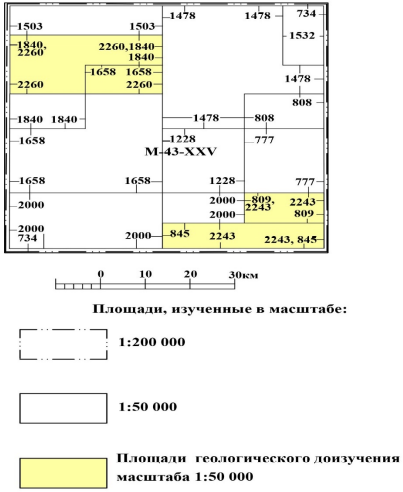
\includegraphics[width=0.6\textwidth]{media/gorn2/image16}
	\caption*{Рис. 1 - Картограмма геологической изученности (лист М-42-XXV)}
\end{figure}

\begin{figure}[H]
	\centering
	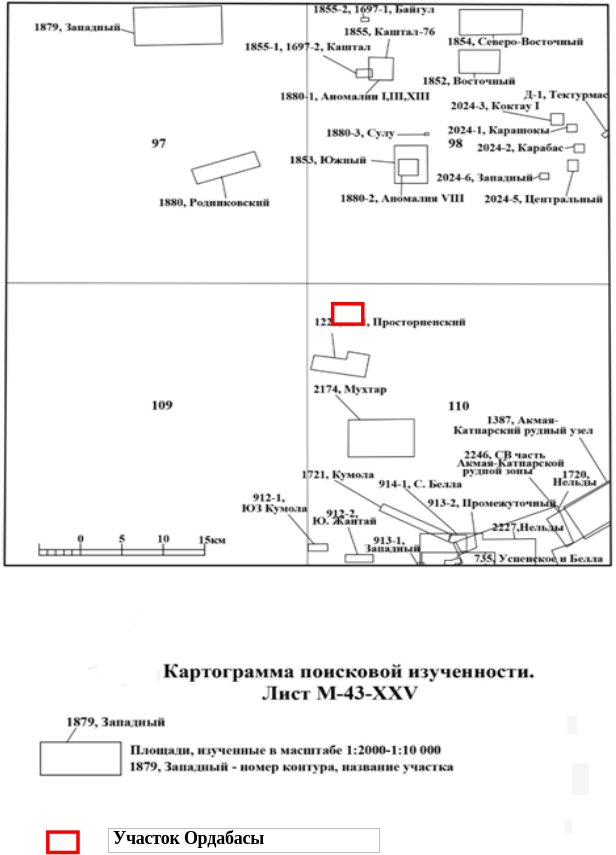
\includegraphics[width=0.6\textwidth]{media/gorn2/image17}
	\caption*{Рис. 2 - Картограмма поисковой изученности}
\end{figure}

\begin{multicols}{2}
Вышеназванными геологами были уточнены и значительно изменены
представления о геологическом строении района и его перспективах в
отношении полезных ископаемых, детализированы стратиграфические схемы
палеозоя, обнаружены органические остатки, собран и обобщен большой
объем петрохимических исследований интрузивных и эффузивных пород.
Впервые в районе выделены каражирикский, прибалхашский и сарджальский
горизонты нижнего девона. Фаунистически охарактеризована тектурмасская
свита кембрия. Допалеозойские отложения расчленены на свиты, толщи и
пачки. Определены перспективы площади на золото, медь, полиметаллы. В
фаменских отложениях установлены фации, перспективные на поиски
свинцово-цинковых руд стратиформного типа, составлена геологическая
карта Атасуйского рудного района.

На основании больших объемов картировочного и поискового бурения
построены карты допалеозойских образований, дробно расчленены отложения
франского, фаменского ярусов и нижнетурнейских отложений с выделением
мелководных и глубоководных фаций; проведено геохимическое исследование
района, выявлены новые проявления рудной минерализации, обоснована
необходимость оценки глубоких горизонтов (более 200 м) медного
месторождения Успенское.

Со второй половины 40-х годов ХХ века по настоящее время на площади
работ ведутся многочисленные инженерно-геологические и
гидрогеологические изыскания, многие из которых связаны с
сельскохозяйственными нуждами (мелиорация земель, обводнение пастбищ).

В период 2004-2007 года Магретовой Л.И. (МД «Центрказнедра») проведены
работы по геологическому доизучению площадей м-ба 1:200000 (ГДП-200) на
территории листов М-42-XXX, М42-XXXVI, M-43-XXV. В процессе полевых
работ авторами пройдено 3664 п.км геологических и поисковых маршрутов,
684 п.км. геолого-геохимических при выполнении специализированных работ
по минерагеническому картированию, 11000 м маршрутов по составлению
опорных стратиграфических разрезов (6 детальных разрезов с отбором
флоры, фауны и проб на силикатный анализ), пробурено 4004 п.м поискового
и 22450 п.м. картировочного бурения, пройдено 3577 м\textsuperscript{3}
поисковых канав.

В западной части листа М-43-XXV на участке Бурминский авторами выполнены
специализированные геолого-минералогические исследования. Описание
гидротермально-метасоматических ассоциаций по шлифам, согласно методике
Беляева Г.М.,~Плющева Е.В.,~Ушакова О.П.В.В. Шатова {[}9{]}, было
составлено сотрудницей Томского политехнического Университета М.И.
Шаминовой. Вся последующая работа, включая составление карт и текста по
участку Бурминскому, а также описание шлифов и составление карты
метасоматических ассоциаций на площадь участка Ордабасы, выполнена
ведущим геологом ТОО «Центргеолсъемка» И.Г. Масловой. Обоснование
возраста выделенных стратиграфических подразделений базируются на
результатах определений 435 точек сборов фауны и флоры, в том числе 109
выявленных при выполнении ГДП-200. Палеонтологические полевые работы
выполнены авторами отчета, а также геологами З.А. Климахиной и Г.В.
Филатовой по договору с АО «Азимут Энерджи Сервисез». Датирование
интрузивных образований основано на результатах 40 геохронологических
определений, выполненных разными исследователями на площади работ в
предыдущие годы. Площадь ГДП-200 располагается в зоне сопряжения 12
разновозрастных структурно-формационных зон Центрального Казахстана и
характеризуется сложным геологическим строением с широким развитием
надвиговых структур и олистостромовых комплексов. Присутствуют
стратифицированные отложения от позднего протерозоя до мезо-кайнозоя и
интрузивные образования (от ультраосновных до ультракислых) в диапазоне
возрастов от позднего рифея до поздней перми.

\emph{Поисковая изученность.} Поисковые и поисково-оценочные работы на
изученной территории проводились как в процессе геолого-съемочных работ
(Рисунок 2), так и в ходе различного рода специализированных поисков. До
50-х годов работы носили эпизодический характер. К этому времени в
Атасуйском районе известны были в основном железомарганцевые проявления
и месторождения, связанные с карбонатными отложениями верхнего девона --
нижнего карбона. Поэтому основное внимание при детальных поисках
уделялось изучению литологии, стратиграфии и структуре этих отложений.
Так, в 1950 году В.Е. Куман проводил разведку проявления марганца
Сулу-Медине и признал его непромышленным, но в отчете автор приводит
дробную стратиграфическую схему осадочных девон-карбоновых отложений,
которая несколько отличается от схемы А.А. Богданова. В 1951 году в
южной части листа М-43-XXV проводились поисковые работы на марганец В.Л.
Саркисяном. Им были выявлены проявления Восточный и Западный Айгыржал и
разведано месторождение Катпар. Железомарганцевое месторождение Большой
Ктай и марганцевое месторождение Керегетас с 1939 года с перерывами
разведывались рядом геологов и в 1955 году В.И. Кавуном разведка их была
завершена. На месторождении Большой Ктай произведен подсчет запасов
железных и марганцевых и железомарганцевых руд. В отношении
полиметаллического оруденения район месторождения получил отрицательную
оценку. На месторождении Керегетас подсчитаны запасы марганцевых и
железомарганцевых руд по категории С\textsubscript{2} и утверждены ВКЗ
СССР {[}10{]}.

Новый этап поисковых работ начался с проведением площадных геофизических
работ масштаба 1:50000, выполнявшихся Агадырской геофизическая
экспедиция (ГФЭ) в 50-60 годах ХХ века.

В 1968 году Агадырской ГФЭ выполнены поисковые работы масштаба 1:10000
на медь и молибден на участке Просторненском. Проявление было выявлено
этой же экспедицией в 1967 году в процессе проведения поисково-съемочных
работ масштаба 1:50000; на нем был выполнен небольшой объем
горно-буровых работ. В результате была установлена
прожилково-вкрапленная редкометалльная и медная минерализация,
приуроченная к малой линейной интрузии гранитов, пронизанных густой
сетью рудоносных кварцевых прожилков. Была выделена значительная (более
1,2 км\textsuperscript{2}) площадь минерализованных пород, что послужило
основанием для продолжения поисковых работ на участке Просторненский.
Оценка оруденения осуществлялась комплексом методов, включающих
магниторазведку, электроразведку, литохимические поиски, горно-буровые
работы. В результате на исследованной площади выделено две рудных зоны:

1. рудная зона, приуроченная к линейной малой интрузии гранитов
субширотного простирания; содержания меди, молибдена и вольфрама
обычно низкие;

2. рудная зона, приуроченная к эндоконтакту Просторненского массива;
породы не изменены, но содержат сеть кварцевых прожилков с пиритом,
халькопиритом и молибденитом.

Кроме рудных зон на площади выявлен ряд геофизических аномалий,
приуроченных к эндо-экзоконтактугранитоидов Просторненского массива и
осадочных пород нижнего силура. Большая часть этих аномалий либо изучена
недостаточно, либо совсем не проверена. НТС ЦКГУ постановило, что
однозначный вывод о промышленной значимости проявления не представляется
возможным, поисковые работы с целью оценки геофизических аномалий
необходимо продолжить, рудные зоны необходимо проследить к западу и
северо-западу от участка комплексом геохимических и геофизических
методов масштаба 1:10000. В 1973-1976 годах В.И. Серегиным (таблица 1)
были проведены поисковые работы на золото на площади проявления Каштал,
выявленного при проведении геолого-съемочных и поисковых работ масштаба
1:50000 Долганевым в 1973 году. На площади 3,5 км\textsuperscript{2}
выполнены магниторазведка, горно-буровые работы. В результате на участке
установлено два типа золотого оруденения: кварцевые жилы с сульфидной
минерализацией и золотом и зоны гидротермально измененных пород с
сульфидами и невысокими содержаниями золота. Запасы золота в кварцевых
жилах были признаны непромышленными, отработка их возможна лишь
старательским способом. Оценку минерализованных зон рекомендовано
продолжить. При проведении общих поисков на территории, прилегающей к
проявлению Каштал, было выявлено новое проявление золота - Байгул.
\end{multicols}

\begin{longtblr}[
  label = none,
  entry = none,
  caption = {\bfseries Таблица 1 - Каталог к картограммам поисковой изученности листов M-43-XXV},
]{
  colspec = {X[0.8] X[1] X[1] X[1] X[1] X[1.2]},
  cells = {c},
  cell{3}{1} = {c=6}{},
  hlines,
  vlines,
}
\textbf{№ контура на картограмме изученности} & \textbf{Фамилия, и., о. автора отчета} & \textbf{Год завершения работ} & \textbf{Организация, проводившая работы} & \textbf{Масштаб работ} & \textbf{Название участка}                             \\
\textbf{1}                                    & \textbf{2}                          & \textbf{3}                   & \textbf{4}                              & \textbf{5}            & \textbf{6}                                           \\
М-43-XXV                                      &                                     &                              &                                         &                       &                                                      \\
735                                           & Гордиенко А.Я.                      & 1959                         & Агад.ГРЭ ЦКГУ                           & Разведочные работы    & Успенское, Белла                                     \\
912-1                                         & Кишко В.М.                          & 1963                         & Агад.ГРЭ ЦКГУ                           & 1:10 000              & Юго-Западная Кумола                                  \\
912-2                                         & Кишко В.М.                          & 1963                         & Агад.ГРЭ ЦКГУ                           & 1:10 000              & Южный Жуманай                                         \\
913-1                                         & Кишко В.М.                          & 1963                         & Агад.ГРЭ ЦКГУ                           & 1:10 000              & Западный                                             \\
913-2                                         & Кишко В.М.                          & 1963                         & Агад.ГРЭ ЦКГУ                           & 1:10 000              & Промежуточный                                        \\
914-1                                         & Кишко В.М.                          & 1963                         & Агад.ГРЭ ЦКГУ                           & 1:10 000              & Северная Белла                                       \\
1229                                          & Малахов В.С.                        & 1967                         & Агад.ГРЭ ЦКТГУ                          & 1:10 000              & Просторненский                                       \\
М-1                                           & Малахов В.С.                        & 1969                         & Агад.ГРЭ ЦКТГУ                          & 1:10 000              & Просторненский                                       \\
1387                                          & Абеуов А.К.                         & 1972                         & Агад.ГРЭ ЦКТГУ                          & 1:10 000              & Акмая-Катпар-ский рудный узел                        \\
1697-1                                        & Серегин В.М.                        & 1976                         & Кар.КГГЭ ЦКТГУ                          & 1:10 000              & Байгул                                               \\
1697-2                                        & Серегин В.М.                        & 1976                         & Кар.КГГЭ ЦКТГУ                          & 1:10 000              & Каштал                                               \\
1720                                          & Овечкин В.Г.                        & 1976                         & Агад.КГГФЭ ЦКТГУ                        & 1:10 000              & Недьды                                               \\
1721                                          & Овечкин В.Г.                        & 1976                         & Агад.КГГФЭ ЦКТГУ                        & 1:10 000              & Кумола                                               \\
1852                                          & Серегин В.М.                        & 1979                         & Кар.КГГЭ ЦКТГУ                          & 1:10 000              & Восточный                                            \\
1853                                          & Серегин В.М.                        & 1979                         & Кар.КГГЭ ЦКТГУ                          & 1:10 000              & Южный                                                \\
1854                                          & Серегин В.М.                        & 1979                         & Кар.КГГЭ ЦКТГУ                          & 1:10 000              & Северо-Восточный                                     \\
1855                                          & Серегин В.М.                        & 1979                         & Кар.КГГЭ ЦКТГУ                          & 1:10 000              & Каштал-76                                            \\
1855-1                                        & Серегин В.М.                        & 1979                         & Кар.КГГЭ ЦКТГУ                          & 1:10 000              & Каштал                                               \\
1855-2                                        & Серегин В.М.                        & 1979                         & Кар.КГГЭ ЦКТГУ                          & 1:10 000              & Байгул                                               \\
1879                                          & Конопаткин А.Я.                     & 1980                         & Кар.ГРЭ ЦКПГО                           & 1:10 000              & Западный                                             \\
1880                                          & Конопаткин А.Я.                     & 1980                         & Кар.ГРЭ ЦКПГО                           & 1:10 000              & Родниковский                                         \\
1880-1                                        & Конопаткин А.Я.                     & 1980                         & Кар.ГРЭ ЦКПГО                           & 1:10 000              & Аномалии I,III,XIII                                  \\
1880-2                                        & Конопаткин А.Я.                     & 1980                         & Кар.ГРЭ ЦКПГО                           & 1:10 000              & Аномалии VIII                                        \\
1880-3                                        & Конопаткин А.Я.                     & 1980                         & Кар.ГРЭ ЦКПГО                           & 1:10 000              & Сулу                                                 \\
Д-1                                           & Девятериков Н.Ф.                    & 1981                         & Кар.ГРЭ ЦКПГО                           & Разведка              & Тектурмас                                            \\
2024-1                                        & Зеленый В.А.                        & 1986                         & Кар.ГРЭ ЦКПГО                           & 1:2 000               & Карашокы                                             \\
2024-2                                        & Зеленый В.А.                        & 1986                         & Кар.ГРЭ ЦКПГО                           & 1:2 000               & Карабас                                              \\
2024-3                                        & Зеленый В.А.                        & 1986                         & Кар.ГРЭ ЦКПГО                           & 1:2 000               & КоктауI                                              \\
2024-5                                        & Зеленый В.А.                        & 1986                         & Кар.ГРЭ ЦКПГО                           & 1:2 000               & Центральный                                          \\
2024-6                                        & Зеленый В.А.                        & 1986                         & Кар.ГРЭ ЦКПГО                           & 1:2 000               & Западный                                             \\
2174                                          & Тевс А.А.                           & 1991                         & Агад.ГРЭ ЦКПГО                          & 1:10 000              & Мухтар                                               \\
2227                                          & Мынбаев М.У.                        & 1994                         & АО «Акбар»                              & 1:10 000              & Нельды                                               \\
2246                                          & Авдеев С.Л.                         & 1994                         & АО «Акбар»                              & 1:50 000,1:2 000      & Северо-Восточная часть Акмая-Кат-парской рудной зоны 
\end{longtblr}

\begin{multicols}{2}
Оценка проявлений Байгул и Каштал горно-буровыми работами была проведена
В.И. Серегиным в 1976-1979 годах. Кроме этого, магниторазведочные и
литохимические поиски масштаба 1:10000 выполнены на участках Каштал-76,
Северо-Восточный, Восточный и Южный, расположенных по периферии
проявления Каштал.

На проявлении Каштал изучались золоторудные зоны в гидротермально
измененных роговиках, залегающих в экзоконтакте
лакколитообразныхинтрузий диоритов. По двум зонам до глубины 200 м
подсчитаны запасы золота категории С\textsubscript{2}.

На проявлении Байгул изучалось золотое оруденение, связанное с
непротяженными кварцевыми жилами сложной морфологии, залегающими внутри
массива диоритов. Запасы золота подсчитывались по категории
С\textsubscript{2}, объект может представлять интерес для старательской
отработки.

Перспективы увеличения запасов авторы связывают с метасоматитами,
развитыми в южном и западном экзоконтакте интрузии диоритов; здесь
получены положительные результаты по работам методом ВП-ВЭЗ. Изучение
зоны авторы рекомендуют продолжить путем бурения скважин глубиной не
менее 200 м.

На участках Северо-Восточный, Восточный, Каштал-76 и Южный
магниторазведкой выявлено до 15 компактных магнитных аномалий,
вызванных, предположительно, малыми интрузиями диоритов, с которыми в
районе связано золотое оруденения. Из этого количества выделено 3
аномалии - I, III,VIII, на площади которых рекомендуется проведение
первоочередных поисково-оценочных работ на золото и аномалия XIII (ореол
рассеяния свинца, цинка, серебра и кадмия, совмещающийся с аномалией
ВП), перспективная на поиски полиметаллического оруденения.

В период с 1976 года по 1980 годы проводилась детальная разведка
Тектурмасского месторождения кварцитов и его флангов На двух участках --
Северном и Южном оконтурено восемь линзообразных и пластообразных
кварцитовых тел, по которым изучено качество сырья и его технологические
характеристики. По мнению авторов в пределах самого месторождения нельзя
рассчитывать на дальнейший прирост запасов; увеличение их возможно за
счет продолжения геологоразведочных работ на участках, расположенных к
юго-западу от Тектурмасского месторождения.

В центральной части Нуринской СФЗ в 1978-1980 годах были проведены
поиски золота. На площади проявления Сулу выполнены поисково-оценочные
работы, опоискованы ранее выявленные, перспективные на золото магнитные
аномалии I, III, VIII, на полиметаллы - аномалия XIII, проведены общие
поиски золота на участках Родниковский и Западный (центральная часть
Нуринской СФЗ) на площади около 400 кв.км. По результатам
поисково-оценочных работ на проявлении Сулу установлено, что жильная
зона прослеживается до глубины 150 м и более без существенного изменения
мощности отдельных кварцевых жил. Запасы до глубины 25 м могут быть
объектом старательской отработки открытым способом. Перспективы
увеличения запасов на глубину маловероятны.

\emph{Тектоника и история геологического развития.} Участок Ордабасы
находится в пределах Сарысуйской структурно-формационной зоны (СФЗ).
Нуринская и Сарысуйская СФЗ -- раннепалеозойские окраинные бассейны,
разделенные Тектурмасским сутурным швом.

Нуринская, Сарысуйская СФЗ -- раннепалеозойские окраинноморские
бассейны, заложенные на энсиматическом основании и разделенные
Тектурмасскимсутурным швом. В период их развития, породы офиолитового
комплекса, слагающие Тектурмасскую СФЗ, слагали вулканическую островную
дугу. Позднее на этом фундаменте была сформирована среднеордовикская
островная дуга, сложенная раннее островодужными толеитовыми
низкокалиевыми и низкотитанистыми базальтами. Ее развитие завершилось
формированием туфогенно-кремнистого базарбайского, сатыбайского и
аирского комплексов {[}11{]}.

Существующая Тектурмасская островная дуга разделила единый бассейн
терригенного осадконакопления на более мелководный Нуринский,
прилегающий к континенту (задуговой) и Сарысуйский, связанный
океаническим бассейном (преддуговой), расположенный южнее (в современных
координатах).

Таким образом, геологические данные, имеющиеся по Казахстанскому
региону, свидетельствуют о том, что в позднем рифее, на уровне 900-800
млн. лет произошел раскол континентов, вслед за которым последовало их
разделение и образование океанического ложа. Очевидно, большая часть
этого ложа формировалась в конце рифея -- венде -- начале кембрия, т.е.
800-550 млн. лет. Параллельно с развитием океана шло формирование
комплексов пассивных окраин, континентального подножия. Существование
океанического бассейна подтверждается наличием глубоководных кремнистых
осадков, накапливающихся, очевидно, ниже уровня карбонатной компенсации
{[}12{]}.

Данный океанический бассейн был частью позднедокембрийско-
раннепалеозойского Палео-Азиатского океана. Начиная с кембрия на
океаническом ложе развиваются островные дуги.

В раннем кембрии возникла Бозшаколь-Чингизская островная дуга, которая
располагалась к западу (в прошлых координатах) от
Казахстанско-Северо-Тяньшанского докембрийского массива. Островная дуга
отгородила от Палео-Азиатского океана часть ложа шириной не менее 1000
км. Океанический бассейн между Бозшаколь-Чингизской островной дугой и
докембрийским массивом можно рассматривать как обширное окраинное море
-- Акдымский бассейн. Его осадочное выполнение осталось в виде
глубоководных кремнисто-фтанитовых и турбидитных толщ (каратасская свита
Атасуйской и акдымская серия Ерментауской СФЗ).

В конце ордовика раннем силуре происходит реорганизация геодинамических
обстановок в Казахстанско-Тяньшанском регионе -- начинается поглощение
ложа Акдымского бассейна в зонах Беньофа Бозшаколь-Чингизской и
возникшей Степняк-Бетпак-Далинской островных дуг. В целом эпоха
растяжения сменяется эпохой сжатия. С позднего ордовика - раннего силура
начинается скучивание, деформации и к концу силура основная масса
Акдымского бассейна уже поглощена. На протяжении всего силура происходит
массовое образование олистостромовых комплексов, зон серпентинитового
меланжа, тектонических покровов и т.д. Столкновение дуг закончилось к
концу силура, и зона Беньофа была «перещелкнута» в новое положение на
край вновь образованной континентальной массы.

Таким образом, каледонский массив Центрального Казахстана представляет
собой аккреционную структуру, возникшую за счет столкновения
докембрийских массивовс Бозшаколь-Чингизской и Степняк-Бетпак-Далинской
островными дугами.

В среднем и позднем палеозое Казахстанско-Северо--Тяньшанский массив
имел размеры не более 1000х1500 км, что сопоставимо с современным о.
Калимантан. Как и этот остров в кайнозое, каледонский массив в
герцинскую эпоху был почти со всех сторон окаймлен зонами субдукции,
которые сопровождались вулканическими поясами. Формирование
разновременных вулкано-плутонических поясов, сменяющих друг друга во
времени и пространстве, является характерной особенностью
Казахстанско-Северо-Тяньшанского массива в среднем и позднем палеозое
{[}13{]}.

Формирование каледонид завершилось деформациями, которые происходили с
конца ордовика до конца силура, после чего вдоль границы вновь
созданного каледонского континента возник окраинно-континентальный
вулкано-плутонический пояс, который считается разделом между
казахстанскими каледонидами и герцинидами. К югу, на большей части
Джунгаро-Балхашской области, континентальное основание отсутствовало.

\emph{Разрывные нарушения}{\bfseries .} Тектурмасская зона разломов --- это
целая серия разломов северо-восточного простирания, куда входят Северо-
и Южно-Тектурмасский надвиги, а также Кужал-Жартасская зона разломов,
где первый надвиг является северным ограничением зоны, а последние --
южным.

В магнитном поле Северо-Тектурмасский и Южно-Тектурмасский разломы
окаймляют полосу локальных положительных аномалий (∆Т)\textsubscript{а}
различной интенсивности до 1500 нТл над породами альпинотипного
комплекса нижнего ордовика
(χ\textsubscript{ср.}=23-2500∙10\textsuperscript{-5}СИ) и трассируются
зонами градиента (∆Т)\textsubscript{а}. А Кужал-Жартасская зона разломов
фиксируется фрагментарно зоной градиента (∆Т)\textsubscript{а} в
северном контакте Просторненского и Итольгенского массивов
гранит-гранодиоритов верхнего девона.

В районе очень четко проявлены надвиговые структуры. В направлении с
юго-востока на северо-запад (перпендикулярно северо-восточным разломом)
происходили надвиговые движения (шарьирование), формирующие серию
(пакет) пластин, отражающих сложное покровно-чешуйчатое строение района
работ.

Надвигание происходило неоднократно, сопровождалось формированием
меланжевых и олистостромовых комплексов. Вероятно, перед формированием
флишевых бассейнов, происходило «захлопывание» океанического бассейна с
формированием мономиктового (из ультраосновных пород) и полимиктового
(из всех пород офиолитовой ассоциации) меланжа. В период накопления
флишоидных толщ в краевых частях бассейна шло образование
олистостромовых комплексов, обусловленное неспокойной тектонической
обстановкой в формирующихся бассейнах, а также происходящим в это время
шарьированием пород офиолитового комплекса. При последующих этапах
надвигообразования в этот процесс были вовлечены и олистостромовые толщи
вместе с меланжевыми образованиями. За счет этого в современной
структуре Тектурмасский офиолитовый пояс имеет покровно-складчатое
строение, в котором практически все первоначальные взаимоотношения
нарушены и он представляет собой: сочетание мономиктового меланжа,
развитого ограниченно и слагающего, видимо, подошвенные части
тектонических пластин; полимиктового меланжа, представляющего собой
скорее тектоническую смесь, состоящую из олистолитов полимиктового
меланжа и олистостромового комплекса, матрикс в котором представлен, как
правило, тонкорассланцованными голубовато-зелеными алевролитами, реже
песчаниками силурийского возраста. В этой смеси характерно присутствие
крупных блоков яшм, базальтов, габброидов, являющихся фрагментами
разновозрастных тектонических пластин.

{\bfseries Результаты и обсуждение.} Все известные на площади работ
месторождения, проявления и пункты минерализации классифицированы по
генетическим типам. Проведен их комплексный анализ, выявлены
минерагенические критерии, поисковые признаки и геологические
предпосылки. Выделены потенциально перспективные площади первой и второй
очереди с указанием категории ожидаемых ресурсов:

- на площади листа М-42-XXX: Айгыржальская железомарганцевая в
кремнистых отложениях каратасской свиты верхнего кембрия--среднего
ордовика и Шоимбайская золото-кварцево-жильная в терригенных отложениях
верхнего силура (I очереди) и Алтынказганская золото-кварцево-жильная в
терригенных образованиях нижнего силура (II очереди);

-на площади листа M-42-XXXVI: в Жаильминской минерагенической зоне --
Кентобе-Бестюбинская барит-полиметаллическая (I очереди); Керегетасская
железо-марганцевая и Ушкагыльская свинцово-цинковая (II очереди) в
карбонатно-кремнисто-терригенных отложениях фаменского возраста;

- на площади листа М-43-XXV: Сулумединская железомарганцевая (I очереди)
в карбонатно-глинистых отложениях турнейского возраста; Просторненская
медно-молибденовая и Ордабасская молибденово-медная (II очереди),
приуроченные к гранитоидам позднедевонского просторненского интрузивного
комплекса.

В свою очередь магнитные аномалии в 1980 годах были оценены бурением
поисково-картировочных скважин глубиной до 50 м, в которых выполнены
исследования методом заряда ВП. В результате работ было установлено, что
магнитные аномалии связаны с мелкими не вскрытыми эрозией интрузивами
диоритов, прорывающих терригенные отложения силура -- нижнего девона.
Вмещающие породы ороговикованы, отмечается тонкопрожилковое
окварцевание, пиритизация. Эта аномалия рекомендуется для проведения
дальнейших поисково-оценочных работ, остальные магнитные аномалии
оцениваются как бесперспективные.

{\bfseries Выводы.} Таким образом, учитывая предварительную оценку ученых и
геологов прошлых лет, и изучив накопленный материал, можно сделать вывод
о перспективности участка Ордабасы. Для дальнейшей оценки
перспективности участка будут проведены поисково-оценочные работы.
Данные работы включают анализ и обобщение геологических данных по
изучаемой территории. Следующим этапом рассматривается геологическое
картирование путем проведения поисковых и рекогносцировочных маршрутов,
а также проведение площадных геофизических исследований --
электроразведка методом ВП-СГ по сети 100х20 м, электроразведка ЗСБ по
сети 100×50 м с шагом 100 м. Предусматривается обязательное проведение
горных и буровых работ по сети 400х400 м со сгущением разведочной сети
до 200 м, и оценка распространения медного оруденения на глубину до 500
м. Отбор технологических проб и проведение анализов. Данные этапы
изучения участка даст возможность подсчета запасов и прогнозных ресурсов
по категории С2+P1+P2 медной руды и сопутствующих компонентов.
\end{multicols}

\begin{center}
{\bfseries Литература}
\end{center}

\begin{references}
1. Самыгин С.Г., Хераскова Т.Н. Геологическое строение и этапы
тектонической эволюции палеозоид Казахстана
//Литосфера.-2019.-Т.19.(3).- С. 347-371.
\href{https://doi.org/10.24930/1681-9004-2019-19-3-347-371}{DOI
10.24930/1681-9004-2019-19-3-347-371}

2. Степанец В. Г., Макат Д. К., Савельева Н. А. Геодинамическая позиция
медно-порфирового месторождения Нурказган (Центральный Казахстан)
//Металлогения древних и современных океанов.- 2015. - №. 1.- С.
120-124.

3. Бекжанов Г. Р. О направлениях геологоразведочных работ на медь в
Казахстане //Геология и охрана недр. - 2012. - № 4. - С. 52-54.

4. Сафонова И. Ю. и др. Геологическое строение и медное оруденение
Тектурмасского офиолитового пояса и смежных территорий Центрального
Казахстана //Литосфера. - 2022. -Т. 22 (4) - С. 472-496.

5. Султанов Г. Д., Вихлянцев А. А., Исмаилов Х. К. Шешенкаринское рудное
поле в Центральном Казахстане: перспективы обнаружения
золото-медно-полиметаллического месторождения //Новое в познании
процессов рудообразования: Девятая Российская молодёжная
научно-практическая Школа с международным участием. - 2019. - С.
413-416. ISBN ~978-5-88918-055-5

6. Гинатулин А. М., Дербас А. Н., Асанбаева У. Т. Состояние восполнения
запасов ведущих полезных ископаемых Республики Казахстан: проблемы и
некоторые пути их решения //Геология и охрана недр. - 2016. -№ 1.- С.
86-91.

7. Канфель О. М., Мазарович О. А., Турсина В. В. Геологическое строение
северного обрамления Карагандинского бассейна. //Вестн. Моск. ун-та.
Сер. 4. Геология. - 1962. - № 6. - С. 19-35.

8. Портнов В.С., Юров В.М., Турсунбаева А.К., Умбетова А.Т. Оценка
прогнозных ресурсов месторождений полезных ископаемых геофизическими
методами //Фундаментальные исследования. - 2012. - № 3(2). - С. 403-408.

9. Плющев Е.В.,Ушаков О.П.,Шатов В.В. Беляев Г.М. Методика изучения
гидротермально - метасоматических образований. -Ленинград: Недра, 1981.
-262 с.

10. Рахманов В. П., Григорьев В. М., Чайковский В. К. Марганценосные
провинции и марганценосные формации на территории СССР //Геология и
геохимия марганца.-Наука. 1982. - С. 5-14.

11. Сейтмуратова Э.Ю., Сайдашева Ф.Ф. Стратиграфия и условия формирования
продуктивных рудоносных формаций позднего палеозоя Казахстана //Известия
НАН РК. Серия геологическая. -2006. - № 4. - С. 11-19.

12. Зоненшайн Л. П., Савостин Л. А. Введение в геодинамику. -М.: Недра,
1979. - 311 с.

13. Зоненшайн Л.П.,~Кузьмин М.И.,~Натапов Л.М. Тектоника литосферных плит
территории СССР. Том I. -М.: Недра, 1990.- 328 с. ISBN 5-247-01859-1
\end{references}

\begin{center}
{\bfseries References}
\end{center}

\begin{references}
1. Samygin S.G., Heraskova T.N. Geologicheskoe stroenie i jetapy
tektonicheskoj jevoljucii paleozoid Kazahstana
//Litosfera.-2019.-T.19.(3).- S. 347-371.
DOI 10.24930/1681-9004-2019-19-3-347-371. {[}in Russian{]}

2. Stepanec V. G., Makat D. K., Savel' eva N. A.
Geodinamicheskaja pozicija medno-porfirovogo \\mestorozhdenija Nurkazgan
(Central' nyj Kazahstan) //Metallogenija drevnih i
sovremennyh okeanov.- 2015. - №. 1.- S. 120-124. {[}in Russian{]}

3. Bekzhanov G. R. O napravlenijah geologorazvedochnyh rabot na
med'{} v Kazahstane //Geologija i ohrana nedr. - 2012. -
№ 4. - S. 52-54. {[}in Russian{]}

4. Safonova I. Ju. i dr. Geologicheskoe stroenie i mednoe orudenenie
Tekturmasskogo ofiolitovogo pojasa i smezhnyh territorij
Central' nogo Kazahstana //Litosfera. - 2022. -T. 22
(4)-- S. 472-496. DOI \\10.24930/1681-9004-2022-22-4-472-496.{[}in
Russian{]}

5. Sultanov G. D., Vihljancev A. A., Ismailov H. K. Sheshenkarinskoe
rudnoe pole v Central' nom \\Kazahstane: perspektivy
obnaruzhenija zoloto-medno-polimetallicheskogo mestorozhdenija //Novoe v\\
poznanii processov rudoobrazovanija: Devjataja Rossijskaja molodjozhnaja
nauchno-prakticheskaja \\Shkola s mezhdunarodnym uchastiem. - 2019. - S.
413-416. ISBN 978-5-88918-055-5. {[}in Russian{]}

6. Ginatulin A. M., Derbas A. N., Asanbaeva U. T. Sostojanie
vospolnenija zapasov vedushhih poleznyh iskopaemyh Respubliki Kazahstan:
problemy i nekotorye puti ih reshenija //Geologija i ohrana nedr. -
2016. -№ 1.- S. 86-91. {[}in Russian{]}

7. Kanfel'{} O. M., Mazarovich O. A., Tursina V. V.
Geologicheskoe stroenie severnogo obramlenija \\Karagandinskogo bassejna.
//Vestn. Mosk. un-ta. Ser. 4. Geologija. - 1962. - № 6. - S. 19-35.
{[}in Russian{]}

8. Portnov V.S., Jurov V.M., Tursunbaeva A.K., Umbetova A.T. Ocenka
prognoznyh resursov \\mestorozhdenij poleznyh iskopaemyh geofizicheskimi
metodami //Fundamental' nye issledovanija. - 2012. - №
3(2). - S. 403-408. {[}in Russian{]}

9. Pljushhev E.V., Ushakov O.P., Shatov V.V. Beljaev G.M. Metodika
izuchenija gidrotermal' \\no-metasomaticheskih obrazovanij.
-Leningrad: Nedra, 1981. -262 s. {[}in Russian{]}

10. Rahmanov V. P., Grigor' ev V. M., Chajkovskij V. K.
Margancenosnye provincii i margancenosnye formacii na territorii SSSR
//Geologija i geohimija marganca.-Nauka. 1982. - S. 5-14. {[}in
Russian{]}

11. Sejtmuratova Je.Ju., Sajdasheva F.F. Stratigrafija i uslovija
formirovanija produktivnyh rudonosnyh formacij pozdnego paleozoja
Kazahstana //Izvestija NAN RK. Serija geologicheskaja. -2006. - № 4. -
S. 11-19. {[}in Russian{]}

12. Zonenshajn L. P., Savostin L. A. Vvedenie v geodinamiku. -M.: Nedra,
1979.- 311 s. {[}in Russian{]}

13. Zonenshajn L.P., Kuz' min M.I., Natapov L.M.
Tektonika litosfernyh plit territorii SSSR. Tom I. -M.: Nedra, 1990.-
328 s. ISBN 5-247-01859-1. {[}in Russian{]}
\end{references}

\begin{authorinfo}
\emph{{\bfseries Сведения об авторах}}

Тұрғали А.Т. - докторант, Каспийский университет технологии и
инжиниринга им. Ш. Есенова, Актау, Казахстан, e-mail:
\href{mailto:aiman.tt@mail.ru}{\nolinkurl{aiman.tt@mail.ru}};

Қожахмет Қ.Ә. - к.г-м.н., асоциированный профессор, Каспийский
университет технологии и инжиниринга им. Ш. Есенова, Актау, Казахстан,
e-mail:
\href{mailto:kossarbay.kozhakhmet@yu.edu.kz}{\nolinkurl{kossarbay.kozhakhmet@yu.edu.kz}};

Гусманова А.Г. - к.т.н., декан факультета, Каспийский университет
технологии и инжиниринга им. Ш. Есенова, Актау, Казахстан, e-mail:
\href{mailto:aigul.gusmanova@yu.edu.kz}{\nolinkurl{aigul.gusmanova@yu.edu.kz}};

\emph{{\bfseries Information about the authors}}

Turgali A.T. - Doctoral student, Caspian University of Technology and
Engineering named after Sh. Yesenov, Aktau, Kazakhstan, e-mail:
\href{mailto:aiman.tt@mail.ru}{\nolinkurl{aiman.tt@mail.ru}};

Kozhakhmet K.A. - Candidate of Geological and Mineralogical Sciences,
Associate Professor, Caspian University of Technology and Engineering
named after Sh. Yesenov, Aktau, Kazakhstan, e-mail:
\href{mailto:kossarbay.kozhakhmet@yu.edu.kz}{\nolinkurl{kossarbay.kozhakhmet@yu.edu.kz}};

Gusmanova A.G. - candidate of Technical Sciences, Dean, Caspian
University of Technology and Engineering named after Sh. Yesenov, Aktau,
Kazakhstan,
\href{mailto:aigul.gusmanova@yu.edu.kz}{\nolinkurl{aigul.gusmanova@yu.edu.kz}};
\end{authorinfo}
